%%%%%%%%%%%%%%%%%%%%%%%%%%%%%%%%%%%%%%%%%%%%%%%%%%%%%%%%%%%%%%%%%%%%%%%%%%%%%%%%%%%%
%Do not alter this block of commands.  If you're proficient at LaTeX, you may include additional packages, create macros, etc. immediately below this block of commands, but make sure to NOT alter the header, margin, and comment settings here. 
\documentclass[12pt]{article}
 \usepackage[margin=1in]{geometry} 
\usepackage{amsmath,amsthm,amssymb,amsfonts, enumitem, fancyhdr, color, comment, graphicx, environ}
\pagestyle{fancy}
\setlength{\headheight}{65pt}
\newenvironment{problem}[2][Problem]{\begin{trivlist}
\item[\hskip \labelsep {\bfseries #1}\hskip \labelsep {\bfseries #2.}]}{\end{trivlist}}
\newenvironment{sol}
    {\emph{Solution:}
    }
    {
    \qed
    }
\specialcomment{com}{ \color{blue} \textbf{Comment:} }{\color{black}} %for instructor comments while grading
\NewEnviron{probscore}{\marginpar{ \color{blue} \tiny Problem Score: \BODY \color{black} }}
%%%%%%%%%%%%%%%%%%%%%%%%%%%%%%%%%%%%%%%%%%%%%%%%%%%%%%%%%%%%%%%%%%%%%%%%%%%%%%%%%
\usepackage[UTF8]{ctex}
\usepackage{ulem}
\usepackage[framed,numbered,autolinebreaks,useliterate]{mcode}
\usepackage{textcomp}
%%%%%%%%%%%%%%%%%%%%%%%%%%%%%%%%%%%%%%%%%%%%%
%Fill in the appropriate information below
\lhead{Name: 陈稼霖\\ StudentID: 45875852}  %replace with your name
\rhead{SI 140 \\ Probability and Statistics \\ Semester Spring 2019 \\ Assignment 6} %replace XYZ with the homework course number, semester (e.g. ``Spring 2019"), and assignment number.
%%%%%%%%%%%%%%%%%%%%%%%%%%%%%%%%%%%%%%%%%%%%%


%%%%%%%%%%%%%%%%%%%%%%%%%%%%%%%%%%%%%%
%Do not alter this block.
\begin{document}
%%%%%%%%%%%%%%%%%%%%%%%%%%%%%%%%%%%%%%


%Solutions to problems go below.  Please follow the guidelines from https://www.overleaf.com/read/sfbcjxcgsnsk/


%Copy the following block of text for each problem in the assignment.
\begin{problem}{1}
Let $U_1,U_2,...,U_{60}$ be i.i.d. Unif(0,1) and $X=U_1+U_2+\cdots+U_{60}$
\begin{enumerate}
    \item which important distribution is the distribution of $X$ very close to? Specify what the parameters are, and state which theorem justifies your choice.
    \item Give a simple but accurate approximation for $P(X>17)$. Justify briefly.
\end{enumerate}
\end{problem}
\begin{sol}
\\1. The distribution of $X$ is very close to \uline{Normal Distribution}, with expectation $\mu=60E(U_i)=60\times\frac{1}{2}=30$ and variance $\sigma^2=60Var(U_i)=60\int_0^1(x-\frac{1}{2})^2dx=5$.\\
\uline{Central Limit Theorem} justifies my choice.\\
2. Approximation: $P(X>17)\approx1$. Justification:
\[
P(X>17)=P(\frac{X-30}{\sqrt{5/60}}>\frac{17-30}{\sqrt{5/60}})\approx\Phi(26\sqrt{3})\approx1
\]
\end{sol}

\begin{problem}{2} 
Let $X$ and $Y$ be Pois($\lambda$) r.v.s. and $T=X+Y$. Suppose that $X$ and $Y$ are not independent, and in fact $X=Y$. Prove or disprove the claim that $T\sim Pois(2\lambda)$ in this scenario.
\end{problem}
\begin{sol}
Disprove:\\
The p.g.f. of X (or Y) is
\[
G_X(z)=\exp[\lambda(z-1)]
\]
Since $T=X+Y$ and $X=Y$,
\[
T=2X
\]
The p.g.f. of T is
\[
G_T(z)=G_{2X}(z)=G_X(z^2)=\exp[\lambda(z^2-1)]
\]
However, the p.g.f. of $Pois(2\lambda)$ should be
\[
G_{Pois(2\lambda)}(z)=\exp[2\lambda(z-1)]
\]
Therefore, $T\sim Pois(2\lambda)$ is \uline{incorrect}.
\end{sol}



%Copy the following block of text for each problem in the assignment.
\begin{problem}{3}
Let $X,Y,Z$ be r.v.s such that $X\sim \mathcal{N}(0,1)$ and conditional on $X=x$, $Y$ and $Z$ are i.i.d. $\mathcal{N}(x,1)$.
\begin{enumerate}
    \item Find the joint PDF of $X,Y,Z$.
    \item By definition, $Y$ and $Z$ are conditionally independent given $X$. Discuss intuitively whether or not $Y$ and $Z$ are also unconditianally independent.
    \item Find the joint $PDF$ of $Y$ and $Z$. You can leave your answer as an integral, though the integral can be done with some algebra (such as completing the square) and facts about the Normal distribution.
\end{enumerate}
\end{problem}
\begin{sol}
\\1. The PDF of $X$ is
\[
f_X(x)=\frac{1}{\sqrt{2\pi}}\exp(-\frac{x^2}{2})
\]
The PDF of $Y|X$ and $Z|X$ are
\begin{align*}
f_{Y|X}(y|x)=&\frac{1}{\sqrt{2\pi}}\exp[-\frac{(y-x)^2}{2}]\\
f_{Z|X}(z|x)=&\frac{1}{\sqrt{2\pi}}\exp[-\frac{(z-x)^2}{2}]
\end{align*}
The joint PDF of $X,Y,Z$ is
\begin{align*}
f_{X,Y,Z}(x,y,z)=&f_X(x)f_{Y,Z|X}(y,z|x)=f_X(x)f_{Y|X}(y|x)f_{Z|X}(z|x)\\
=&\frac{1}{(2\pi)^{3/2}}\exp[-\frac{x^2+(y-x)^2+(z-x)^2}{2}]
\end{align*}
2. Intuitively speaking, $Y$ and $Z$ are \uline{not} unconditionally independent.\\
3. The joint PDF of (Y,Z) is
\begin{align*}
f_{Y,Z}(y,z)=&\int_{-\infty}^{+\infty}f_{X,Y,Z}(x,y,z)dx\\
=&\int_{-\infty}^{+\infty}\frac{1}{(2\pi)^{3/2}}\exp[-\frac{3x^2-2(y+z)x+y^2+z^2}{2}]dx\\
=&\frac{1}{(2\pi)^{3/2}}\exp[-\frac{y^2+z^2}{2}]\int_{-\infty}^{+\infty}\exp[-\frac{3x^2-2(y+z)x}{2}]dx\\
=&\frac{1}{(2\pi)^{3/2}}\exp[-\frac{y^2+z^2}{2}]\int_{-\infty}^{+\infty}\exp[-\frac{[\sqrt{3}x-\frac{(y+z)}{\sqrt{3}}]^2}{2}+\frac{(y+z)^2}{6}]dx\\
=&\frac{1}{2\sqrt{3}\pi}\exp[-\frac{y^2+z^2-xy}{3}]\int_{-\infty}^{+\infty}\frac{1}{\sqrt{2\pi}}\exp[-\frac{[\sqrt{3}x-\frac{(y+z)}{\sqrt{3}}]^2}{2}]d(\sqrt{3}x)\\
=&\frac{1}{2\sqrt{3}\pi}\exp[-\frac{y^2+z^2-xy}{3}]
\end{align*}
\end{sol}




%Copy the following block of text for each problem in the assignment.
\begin{problem}{4}
A large freight elevator can transport a maximum of 9800 pounds. Suppose a load of cargo containing 49 boxes must be
transported via the elevator. Experience has shown that the weight of boxes of this type of cargo follows a distribution with
mean $\mu$  = 205 pounds and standard deviation $\sigma$  = 15 pounds. Based on this information, what is the probability that all 49
boxes can be safely loaded onto the freight elevator and transported?
\end{problem}
\begin{sol}
Let weight of $i$-th box be $X_i$ and the total wight of the 49 boxes be $S_n$.
\[
S_n=\sum_{i=1}^{49}X_i
\]
We can approximately regard $S_n$ as normal distribution with expectation of $49\mu=10045$ and variance of $49\sigma^2=11025$, so the probability that all 49 boxes can be safely loaded onto the freight elevator and transported is
\[
P(S_n\leq9800)=P(\frac{S_n-10045}{\sqrt{11025}}\leq\frac{9800-10045}{\sqrt{11025}})=\Phi(-\frac{7}{3})=0.009815
\]
\end{sol}


\begin{problem}{5}
In this experiment we will sample 500 samples from probability distribute function $f(x)$. Using the 500 outcomes we will compute the
sample mean . We will repeat until we obtain 1000 values of $ \bar{X}$.\\
1).Plot the histogram of X.\\
2).Plot the histogram of $\bar{X}$.

\begin{figure}[h]
\centering
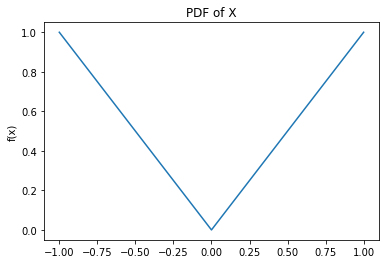
\includegraphics[width=0.4\textwidth]{hw7.png}
\end{figure}
\end{problem}

\begin{sol}
\newpage
1)
\begin{figure}[h]
\centering
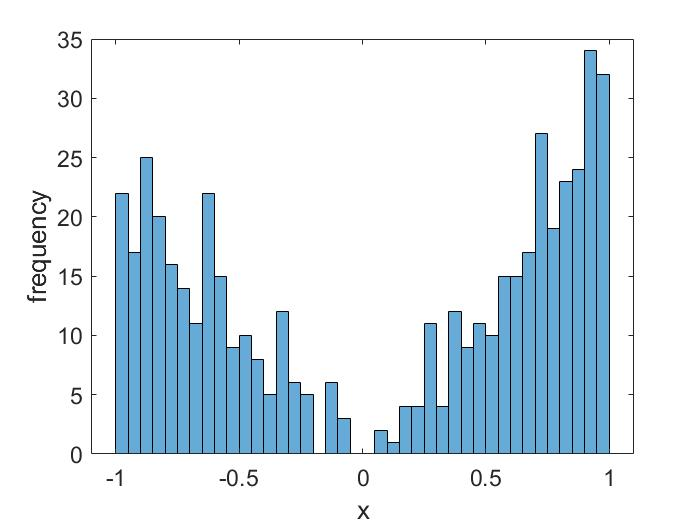
\includegraphics[width=0.7\textwidth]{x_histogram.jpg}
\caption{The histogram of $x$}
\end{figure}

2)

\begin{figure}[h]
\centering
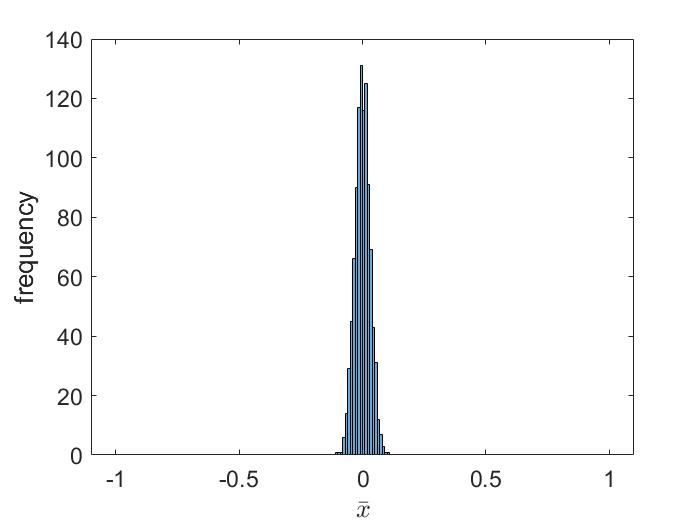
\includegraphics[width=0.9\textwidth]{xbar_histogram.jpg}
\caption{The histogram of $\bar{x}$}
\end{figure}
\end{sol}

\newpage
\textbf{MATLAB代码}
\begin{lstlisting}
close all;clear;clc;
x = zeros(500,1);
x_bar = zeros(1000,1);
for i = 1:1000
    for j = 1:500
        x(j) = f5(rand);
    end
    x_bar(i) = mean(x);
end
figure(1);
histogram(x,'BinEdges',-1:0.05:1);
xlabel('x');
ylabel('frequency');
figure(2);
histogram(x_bar,'BinEdges',-1:0.01:1);
xlabel('$\bar{x}$','Interpreter','LaTeX');
ylabel('frequency');
function y = f5(x)
    % mapping Unif(0,1) to f(x)
    y = sign(x - 1 / 2) .* sqrt(abs(2 * x - 1));
end
\end{lstlisting}
%Copy the following block of text for each problem in the assignment.
%%%%%%%%%%%%%%%%%%%%%%%%%%%%%%%%%%%%%%%%
%Do not alter anything below this line.
\end{document}